\section{Library Implementation}

The library is implemented as three separate components: \emph{i}) runtime code for SPEs, \emph{ii}) basic runtime code for the PPE, and \emph{iii}) runtime code for the PPE that handles extended operations.

\subsection{PPE Implementation}

For each SPE, the library maintains a fixed table of command groups in memory. Each entry in the table represents a group and stores command data for commands in the group. When the user issues a group to an SPE, the library sends a mailbox message to the SPE to notify it of the entry in the table that contains the group and the LS address to copy command data to; the use of a fixed table is directly necessary to be able to pack all required fields into a single 32-bit mailbox message. After receiving the mailbox message, library code on the SPE initiates DMA to copy command data into local store.

When commands are completed by an SPE, library code on the SPE sends a bitmap of the command ID(s) to the PPE via the outbound mailbox. If the mailbox is full (the PPE has not had time to respond to the previous message), the bitmap is queued and sent when the mailbox is empty. The size of a mailbox message (32 bits) currently imposes a strict limit on the range of valid command IDs.

Library code on the PPE continually polls the outbound mailboxes of all SPEs in round-robin order for command completion messages. When a message is received, it is processed by the library, which eventually runs the user-registered callback. Interrupts were not used as each interrupt requires approximately 7 $\mu$s of kernel time to process. Although this may be negligible when only a single SPE is involved, it can become significant when multiple SPEs are all generating interrupts. In general, it is the author's opinion that the Cell architecture's focus on directly using SPEs to run small pieces of application code is not suited for the additional system overhead of interrupts.

One major drawback of the continuous polling approach is that it severely constrains any other work that the PPE is able to perform unless the user is willing to call the library function that performs polling at regular intervals. This is not a problem when the PPE is used solely as a control processor; most control computations are in response to command completion messages from SPEs and can be done in the callback.

The sequence of events that occurs on the PPE and an SPE between the time the user issues a group of commands and the user being notified of the completion of a command in the group via callback is illustrated in figure~\ref{fig:lib:control}. In actuality, because \emph{i}) each SPE is issued multiple commands and \emph{ii}) the PPE is controlling multiple SPEs, there will typically be many different copies of this sequence interleaved within each other, for both the same and different SPEs.

\begin{figure}[!htb]
\begin{center}
\begin{tabular}{rp{2.5in}p{2.5in}}
& \emph{PPE} & \emph{SPE} \\
\cline{2-3}
& Continually polls for command completion messages from SPEs. & Continually polls for mailbox messages while running active commands. \\
\cline{2-3}
\textsf{(1)} & \emph{User creates new group and adds commands.} Command data is written to entry in groups table. & \\
& \emph{User issues group.} Sends mailbox message to SPE. & \\
& & Receives and unpacks mailbox message. Copies command data (using DMA) from table entry to local store at specified LS address. \\
& & After copying command data, adds new commands to dependency graph. \\
& & \multicolumn{1}{c}{$\cdots$} \\
& & When command(s) complete, writes bitmap of completed ID(s) to PPE. \\
& Receives command completion message and calls user-defined callback. & \\
& \emph{Inside callback, user sets up and issues new groups if desired.} Repeats from \textsf{(1)}. &
\end{tabular}
\end{center}
\caption[SPE control protocol.]{SPE control protocol. \emph{Italicized} text represents actions performed by user code. All other actions are performed by library code.}
\label{fig:lib:control}
\end{figure}

\subsection{SPE Implementation}

To execute multiple active commands concurrently on an SPE, the library implements what is effectively a simple co-operatively multitasked ``operating system''. Each type of command has an associated handler function that processes it, and all active commands on an SPE act as separate ``threads'' executing at separate points in their handler functions, using command data to store temporary state in lieu of a separate stack.

The library maintains a run list that contains all active commands in a circular linked list. At the top level, the library cycles through each command in the run list and calls its handler. Each handler performs a small amount of work, typically only part of the work the command specifies, and then returns to the run list to allow other commands to execute. For example, the handler for the \textsf{filter\_run} command runs the filter's work function for one iteration\footnote{To reduce library overhead for filters that have small work functions, the command actually accepts an additional parameter that specifies the number of iterations to run the work function in each cycle through the run list. Alternatively, the compiler can coarsen the work function directly.} and then returns, relinquishing control of the SPE to other commands; in total, the filter's work function is run once for every cycle through the run list. More complex command handlers, such as those for data transfer commands, implement a simple state machine, storing state variables in temporary space in command data. Commands that are queued (have dependencies that have not yet completed) are not placed on the run list and incur no overhead for commands that are running; this allows the user to queue commands according to convenience, with no penalty.

Commands that perform DMA, such as data transfer commands, can wait for DMA operations to complete after starting them. While waiting, the command is removed from the run list, incurring no overhead for commands that are still running. The SPE continues to run other active commands while the DMA is in progress, providing communication--computation concurrency. Once the DMA operation completes, the command is re-added to the run list and the state machine in the command handler will continue where it left off.

DMA completions and inbound mailbox messages are checked via polling instead of interrupts. The library framework allows this internal functionality to be implemented simply as other commands:
\begin{itemize}
\item A command that polls for DMA completions and wakes other commands. This command also sends queued command completion messages to the PPE.
\item A command that polls the inbound mailbox for new command groups from the PPE. This command must perform DMA to copy command data for the group into local store, and does so using the standard mechanism.
\end{itemize}

The library framework causes polling to be done once every cycle through the run list.

From an implementation perspective, the framework does not seem to add significant complexity. In particular, the handlers for data transfer commands have a number of states and consist of a large outer \textsf{switch} statement. However, data transfers, which involve waits, would be fairly complex in any case, and the only obfuscation forced by the framework is that the otherwise linear structure of the handler function is broken up by \textsf{switch} cases. The framework has the advantage of treating all commands uniformly -- any command handler can perform a data transfer -- and thus it allows the library to be easily extended with new commands.

From an efficiency perspective, the run list involves multiple branches that cannot be predicted and does add some overhead to an SPE's main task of running filter work functions. However, this is generally a small fraction of the time spent in even slightly computation-intensive work functions. The run list framework is also not fair in scheduling multiple \textsf{filter\_run} commands: instead of sharing the SPE equally, they are given time proportional to the time spent in a single iteration of their work functions. However, even a single active \textsf{filter\_run} command makes full use of an SPE, and there is commonly only a single running filter (in addition to data transfer commands).

The library completely avoids interrupts, and consequently relies on co-operative multitasking. This was done for a number of reasons. Foremost, the granularity of a filter work function, which typically performs a small amount of work, provides a natural unit of time for switching between commands. SPEs have no timer interrupt; regardless, no timer interrupt could provide the granularity required: a work function of a typical filter might take tens of microseconds to run. In addition, the large number of registers on SPEs makes register saving and restoring time-consuming if interrupts were to be used for DMA completions and inbound mailbox messages. The current framework also avoids any possibility of race conditions when implementing data transfer commands that access buffers: when a data transfer command handler is executing, all filters are between work function iterations and it is the only code accessing the buffer's head and tail pointers.

Since polling is done only at one specific point in the run list, additional latency is introduced into commands that perform DMA. However, this has no effect as long as the user can overlap data transfer commands with computation.
 
Library code occupies approximately the first 16 KB of local store. The remainder is available for use by filter code, filter state, buffers, and the stack.

\subsection{Data Transfer Implementation}

Data transfer between two buffers on different processors involves additional synchronization between the processors. In particular, the source processor communicates to the destination SPE (SPE to memory data transfer will be discussed later later) \emph{i}) that data is available in the source buffer and \emph{ii}) the value of the source buffer's head pointer, so the destination buffer knows where to copy data from. The interaction between a pair of corresponding data transfer commands is given in figure~\ref{fig:lib:dt}:

\begin{figure}[!htb]
\begin{center}
\begin{tabular}{p{2.5in}p{2.5in}}
\emph{Source} & \emph{Destination} \\
\hline
Writes head pointer (using DMA) to destination buffer's control block. & Polls for head pointer from source processor. \\
Polls for acknowledgement from destination SPE. & \\
& After receiving head pointer, starts DMA for actual data. \\
& After copying all data, writes acknowledgement to source buffer's control block. \\
After receiving acknowledgement, completes. & After write completes, completes.
\end{tabular}
\end{center}
\caption{SPE--SPE data transfer protocol.}
\label{fig:lib:dt}
\end{figure}

The actual copying of data is done in a ``pull'' manner by the destination SPE. The entire transfer may require more than one DMA operation when the total transfer size is larger than Cell's maximum 16 KB DMA size, or when either buffer wraps around. After starting a single DMA operation, the destination SPE waits for it to complete before starting the next (during this time, the command is removed from the run list and incurs no overhead).

Polling on both processors is done by checking the control block in the command handler and, if not successful, immediately returning to the run list. The next poll occurs when the command handler is run again the next time through the run list.

Transfers where the source buffer is located in memory (and thus handled by the PPE) differ slightly from the protocol presented above. The PPE can use the completion of the data transfer command on the destination SPE as the acknowledgement.

Transfers where the destination buffer is located in memory require separate handling. Although the PPE can start DMA operations from SPE local store, PPE-initiated DMA is less efficient and having PPE code handle transfers places an additional load on the PPE, which must service all SPEs. Instead, transfers to memory are performed in a ``push'' manner that is approximately the reverse of the protocol described above. The PPE uses the completion of the data transfer command on the source SPE as the acknowledgement; in this manner, polling other than for command completion messages is completely avoided on the PPE and multiple transfers to/from memory place no extra overhead on the PPE.

A single active data transfer command on an SPE does not make full use of the MFC, since it starts a single DMA operation and waits for it to complete before starting another. However, this is offset by two considerations: \emph{i}) there should typically be at least two active data transfer commands, one for the input and one for the output buffers and \emph{ii}) when double-buffering is done via the dependency graph, the slight increase in data transfer latency should have no effect.

For double-buffering to be successful, a \textsf{filter\_run} command that is active concurrently with data transfer commands must return to the run list enough times for the data transfer commands to be able to run completely. As a consequence, \textsf{filter\_run} commands should specify at least three or four iterations. In practice, most filter work functions produce and consume relatively small amounts of data per iteration, and this can be easily met even with relatively small buffer sizes.

%% \subsubsection{Unaligned Data Transfers}

%% Data transfers that do not begin on a quadword boundary\footnote{Where the head pointer of the source buffer and the tail pointer of the destination buffer are not aligned on a quadword.} require special handling, since the Cell architecture requires DMA operations of quadword size or larger to be quadword-aligned. It is not safe to DMA the entire quadword that contains the source buffer's head pointer directly into the destination buffer, since this overwrites data before the end of the destination buffer with data from before the front of the source buffer, which may be invalid (figure~\ref{fig:lib:dtua}a). Treating the unaligned portion of this quadword as a series of 1-, 2-, 4-, and 8-byte DMA operations (figure~\ref{fig:lib:dtua}b) produces a large amount of DMA overhead and is a poor use of Cell's communication network.

%% \begin{figure}[!htb]
%% \begin{center}
%% 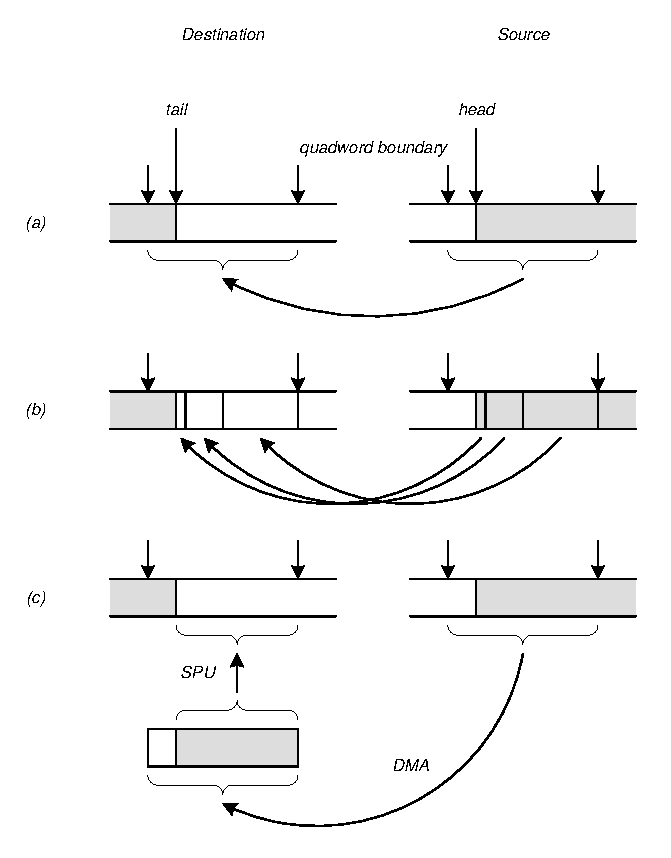
\includegraphics{figs/dt}
%% \end{center}
%% \caption[Different ways of handling unaligned data transfers.]{Different ways of handling unaligned data transfers. (a) is incorrect, since it overwrites data in the destination buffer with invalid data from the source buffer. (b) is correct but involves many DMA operations, and is less efficient. (c) is the actual method implemented.}
%% \label{fig:lib:dtua}
%% \end{figure}

%% Instead, the destination SPE DMAs the quadword from the source buffer into the destination buffer's control block, instead of directly into the buffer. When the DMA completes, the destination SPE writes only the valid portion of quadword into the destination buffer.\footnote{This is actually a read-modify-write operation, but it is done by the SPU, not the MFC.} This is illustrated in figure~\ref{fig:lib:dtua}c. The library uses intrinsics to avoid an expensive \textsf{for} loop. For transfers to a destination buffer located in memory, the source SPE DMAs the quadword to the destination buffer's control block and the PPE writes the valid portion of the quadword into the destination buffer using VMX intrinsics after the source command completes.
